% Ubah judul dan label berikut sesuai dengan yang diinginkan.
\section{Hasil dan Pembahasan}
\label{sec:hasilpembahasan}

% Ubah bagian-bagian berikut dengan isi dari pengujian dan analisis
Pada penelitian ini dipaparkan hasil pengujian serta analisis yang dilakukan sesuai dengan desain sistem yang sudah dirancang pada bab sebelumnya. Dataset yang digunakan berasal dari \url{data.mendeley.com} ditambah dengan dataset yang berasal dari proses \textit{webcrawling} sendiri. Pengujian dilakukan dengan beberapa bagian sebagai berikut :

\begin{enumerate}[nolistsep]
    \item Pengujian performa berdasar pada penggalan kata yang diambil
    \item Pengujian performa berdasarkan model BERT yang digunakan
    \item Pengujian performa berdasarkan pada metode \textit{transformer} yang digunakan.
    \item Pengujian performa berdasarkan pendekatan cara \textit{training}.
\end{enumerate}

Pada pengujian, masing - masing model menggunakan Google Collab dengan spesifikasi \textit{hardware} seperti yang dilampirkan pada tabel \ref{tab:specs_collab}

\begin{table}[h]
    \caption{spesifikasi PC yang digunakan}
    \label{tab:specs_collab}
    \centering
    \begin{tabular}{|l|l|}
        \hline
        \textbf{Prosessor}            & 2 v-core Intel(R) Xeon(R) CPU @ 2.20GHz   \\ \hline
        \textbf{RAM}                  & Virtual Memory : 12GB                     \\ \hline
        \textit{\textbf{Storage}}     & SSD : 69GB                                \\ \hline
        \multirow{2}{*}{\textbf{GPU}} & Nvidia Tesla T4 16GB                      \\ \cline{2-2}
                                      & Nvidia K80 12GB                           \\ \hline
        \textbf{Sistem Operasi}       & Ubuntu 18.04.5 LTS (Bionic Beaver) 64-bit \\ \hline
    \end{tabular}
\end{table}

\subsection{Pengujian performa berdasar pada penggalan kata yang diambil}

Untuk saat ini, BERT hanya dapat memproses sebanyak 512 token sekaligus. Sehingga, untuk melakukan pemprosesan pada data dengan teks yang panjang, diperlukan pemotongan teks agar panjang teks menjadi sesuai.

Pengujian performa berdasar pada penggalan kata yang diambil ini bertujuan untuk mengetahui tingkat akurasi model BERT pada teks dengan cara pemotongan yang berbeda. Pembedaan ini dilakukan berdasarkan pada adanya berita yang menuliskan kesimpulan di awal, atau bisa juga menuliskan kesimpulan di akhir. Alternatif lain adalah mengambil sebagian teks di bagian awal dan mengambil sisanya di bagian akhir. Maka dari itu, dalam pengujian performa ini dilakukan dengan membagi teks pada beberapa cara memenggal kata, dengan rincian sebagai berikut :

\begin{enumerate}
    \item Mengambil bagian awal teks

          Terdapat beberapa ciri - ciri yang terdapat pada kebanyakan teks berita berbahasa Indonesia, salah satu dari ciri - ciri tersebut adalah menuliskan ringkasan berita pada paragraf awal kalimat. Format seperti ini biasanya cukup sering ditemui terutama pada berita yang memanfaatkan fitur halaman pada teks beritanya. Karenanya, pada jenis - jenis berita seperti ini, orang hanya perlu melihat beberapa kalimat awal untuk mengetahui apakah bahwa berita tersebut valid dan dapat dipercaya.

    \item Mengambil bagian akhir teks

          Mirip seperti pengujian dengan mengambil bagian awal teks, terdapat ciri - ciri lain yang biasanya terdapat pada teks berita berbahasa Indonesia adalah adanya kesimpulan pada bagian akhir teks berita. Sehingga, setelah isi berita yang biasanya dibahas cukup dalam, pembaca dapat mengetahui bagaimana dan apa hubungan setiap informasi yang disajikan dengan peristiwa yang sedang dibahas dalam berita.

    \item Mengambil 129 token dari bagian awal teks dan 383 token dari bagian akhir teks

          Pengujian ini berdasarkan pada penelitian Chi Sun et al. yang menemukan bahwa dengan strategi pengambilan teks yang dibagi dua seperti ini akan dapat memberikan nilai akurasi yang lebih baik apabila dibandingkan dengan mengambil hanya di bagian awal maupun di bagian akhir saja \cite{sun2019fine}. Alasan dari penyebab lebih tingginya akurasi adalah karena dengan mengambil sebagian di awal maka sebagian dari ringkasan berita akan didapatkan, sedangkan mengambil sebagian di akhir adalah agar kesimpulan berita juga masuk ke dalam proses \textit{training}. Namun, pengujian tersebut dilakukan pada dataset teks berita berbahasa Inggris sehingga masih harus dilakukan pengujian lagi pada dataset teks berita berbahasa Indonesia.

\end{enumerate}

Dari total data yang berjumlah 1621 data, akan diambil 18\% nya sebagai dataset pengujian, sehingga berjumlah 292 dataset sebagai pengujian. Parameter pada pengujian untuk \textit{training} di atur agar sama untuk setiap pengujian, \textit{epoch} sebesar 7, \textit{leearning rate} sebesar 2e-5, dan \textit{epsilon} sebesar 1e-8, hal yang sama juga dilakukan pada model, pengujian ini menggunakan model BERT yang telah di-\textit{pre-trained} oleh Indobert. Untuk lebih jelasnya, silahkan lihat Tabel \ref{tab: truncate_param} yang berisi rincian parameter dan model yang digunakan untuk proses \textit{training}.

\begin{table}[h]
    \caption{Konfigurasi Parameter Untuk Pengujian berdasarkan Pemotongan Kata}
    \label{tab: truncate_param}
    \centering
    \begin{tabular}{|l|l|}
        \hline
        \textit{\textbf{epoch}}          & 3                              \\ \hline
        \textit{\textbf{learning rates}} & 2e-5                           \\ \hline
        \textit{\textbf{epsilon}}        & 1e-4                           \\ \hline
        \textbf{model}                   & indobenchmark/indobert-base-p1 \\ \hline
    \end{tabular}
\end{table}

Keluaran dari model akan dibandingkan dengan label pada dataset, yang kemudian akan dihitung untuk menghasilkan \textit{confusion matrix}, \textit{recall, precision, accuracy} dan \textit{f1-score} sesuai dengan rumus yang telah dijelaskan sebelumnya.

\begin{table}[h]
    \centering
    \caption{Performa pada pengujian berdasar pada lokasi pemotongan kata}
    \label{tab: truncate_result}
    \begin{tabular}{|p{.12\textwidth}|l|l|l|l|}
        \hline
        \textbf{lokasi pemotongan}      & \textit{\textbf{recall}} & \textit{\textbf{precision}} & \textit{\textbf{f1-score}} & \textit{\textbf{accuracy}} \\ \hline
        awal                            & \textbf{89\%}            & \textbf{90\%}               & \textbf{89\%}              & \textbf{89\%}              \\ \hline
        akhir                           & 88\%                     & 85\%                        & 86\%                       & 86\%                       \\ \hline
        gabungan (129 awal + 383 akhir) & 88\%                     & 88\%                        & 88\%                       & 87\%                       \\ \hline
    \end{tabular}
\end{table}

Seperti bisa dilihat pada tabel \ref{tab: truncate_result}, metode pemotongan teks dengan hanya mengambil bagian awal saja memiliki tingkat akurasi yang paling tinggi dan memiliki nilai \textit{recall} dan \textit{precision} yang seimbang. Hal ini berbeda dengan apabila dilakukan pemotongan pada bagian akhir teks yang menunjukkan ada kemungkinan lebih besar bagi model untuk mengklasifikasi suatu teks berita termasuk ke dalam berita palsu. Metode pemotongan yang menggabungkan 129 token dari awal dan 383 token dari bagian akhir teks memiliki rasio nilai \textit{recall} dan \textit{precision} yang bagus juga sama seperti rasio nilai pada pemotongan pada bagian awal teks, namun, secara isi nilai masih kalah.

\subsection{Pengujian performa berdasarkan model BERT yang digunakan}

Terdapat banyak sekali model BERT yang sudah dibuat oleh berbagai orang di internet, ada model yang memiliki kemampuan \textit{multilanguage} sehingga bisa digunakan di berbagai bahasa sekaligus, namun kebanyakan model yang beredar adalah model yang menggunakan bahasa yang spesifik. Hal ini karena waktu \textit{pre-training} yang lebih singkat karena dataset yang lebih sedikit apabila dibandingkan model dengan kemampuan \textit{multilanguage} dan karena waktu \textit{pre-training} lebih sedikit, maka sumber daya yang digunakan juga menjadi lebih sedikit. Selain itu, dan hal ini adalah yang paling penting, hasil akurasi dari model yang hanya menggunakan 1 bahasa memiliki tingkat akurasi yang lebih tinggi apabila dibandingkan dengan model dengan banyak bahasa sekaligus. Maka dari itu, kami menggunakan beberapa model dengan rincian sebagai berikut :

\begin{enumerate}
    \item bert-base-bahasa-standard-case \textit{(bert-bahasa)}

          Merupakan model BERT yang dibuat oleh huzeinzol05. Model ini hanya mendukung bahasa Melayu, namun pembuat model ini mengklaim bahwa model yang telah dibuat dapat digunakan untuk bahasa melayu maupun bahasa Indonesia karena kesamaan tata bahasa dan arti. Model dilatih pada dataset yang diambil dari Wikipedia berbahasa melayu, Wattpad, dan sosial media \cite{Malaya}.

    \item bert-base-multilingual-uncased \textit{(bert-base)}

          Model BERT ini adalah model dasar yang dibuat langsung oleh tim di Google. Model inilah yang merupakan hasil dari penelitian yang sudah dibuat oleh devlin et al dalam penelitian awal mengenai metode BERT ini. Dilatih menggunakan seluruh data yang dimiliki oleh Wikipedia, sehingga salah satu kelebihan dari model ini adalah kemampuannya dalam mendukung 104 bahasa sekaligus \cite{devlin2019bert}.

    \item indobert-base-p1 \textit{(indobert)}

          Model BERT ini adalah salah satu model BERT yang spesifik mendukung bahasa Indonesia. Model ini dibuat oleh indobenchmark sebagai bagian dari penelitian untuk uji \textit{benchmarking} pada \textit{Natural Language Understanding} (NLU) berbahasa Indonesia. Diantara model - model BERT khusus bahasa Indonesia yang lain, model ini adalah model yang dilatih pada dataset terbanyak, yaitu sebesar 23 GB lebih data yang berasal dari berbagai sumber seperti Wikipedia, Twitter, OpenSubtitle, dan banyak lagi \cite{wilie2020indonlu}.

    \item bert-base-indonesian-522M \textit{(cahya-522M)}

          Model BERT yang spesifik mendukung hanya bahasa Indonesia yang dibuat oleh Cahya Wirawan. Model ini dilatih menggunakan 522M data yang semuanya berasal dari Wikipedia. Merupakan model dengan jumlah \textit{pretrained} dataset yang paling sedikit dibandingkan model - model yang lainnya.

    \item bert-base-indonesian-1.5G \textit{(cahya-1.5G)}

          Sama seperti model sebelumnya, model ini juga dibuat oleh Cahya Wirawan. Yang menjadi pembeda dengan model sebelumnya adalah adanya penambahan dataset sebesar 1G dari situs - situs berita berbahasa Indonesia yang membuat total dataset yang digunakan pada waktu \textit{pre-trained} adalah sebesar 1.5G

\end{enumerate}

\begin{table}[h]
    \centering
    \caption{Konfigurasi yang digunakan oleh model BERT yang digunakan}
    \label{tab:multi_bert_config}
    \begin{tabular}{|p{.5\linewidth}|c|l|p{.12\linewidth} |}
        \hline
        Model                          & epoch & dropout & learning rates \\ \hline
        bert-base-bahasa-standard-case & 4     & 0.2     & 2e-5           \\ \hline
        bert-base-multilingual-uncased & 4     & 0.2     & 2e-5           \\ \hline
        indobert-base-p1               & 3     & 0.1     & 2e-5           \\ \hline
        bert-base-indonesian-522M      & 3     & 0.1     & 2e-5           \\ \hline
        bert-base-indonesian-1.5G      & 3     & 0.2     & 2e-5           \\ \hline
    \end{tabular}
\end{table}

Untuk melakukan \textit{training}, sebelumnya kami mengatur konfigurasi yang akan digunakan oleh model BERT yang sudah disiapkan. Tabel \ref{tab:multi_bert_config} adalah rincian konfigurasi yang kami gunakan pada setiap model. Terdapat beberapa perbedaan pada konfigurasi seperti jumlah \textit{epoch} dan jumlah \textit{dropout}. Hal ini karena apabila menggunakan parameter yang sama untuk setiap model, terdapat model yang mengalami \textit{overfitting} dan ada juga model yang dirasa belum optimal.

\begin{table}[h]
    \centering
    \caption{Tingkat Akurasi dari seluruh model BERT yang digunakan}
    \label{tab:model_bert_result}
    \begin{tabular}{|l|l|l|l|l|p{.12\linewidth}|}
        \hline
        \textbf{model} & \textit{\textbf{recall}} & \textit{\textbf{precision}} & \textit{\textbf{f1-score}} & \textit{\textbf{accuracy}} & \textbf{avg. training time} \\ \hline
        bert-bahasa    & 89\%                     & 82\%                        & 85\%                       & 85\%                       & 03:43                       \\ \hline
        bert-base      & \textbf{97\%}            & 75\%                        & 85\%                       & 86\%                       & 02:07                       \\ \hline
        indobert       & 89\%                     & \textbf{90\%}               & \textbf{89\%}              & \textbf{89\%}              & 02:05                       \\ \hline
        cahya-522M     & 88\%                     & 80\%                        & 84\%                       & 84\%                       & \textbf{02:03}              \\ \hline
        cahya-1.5G     & 93\%                     & 80\%                        & 86\%                       & 87\%                       & 02:08                       \\ \hline
    \end{tabular}
\end{table}

Dari tabel \ref{tab:model_bert_result}, dapat disimpulkan bahwa apabila suatu model BERT menggunakan dataset yang sedikit pada waktu \textit{pre-training}, maka waktu yang diperlukan untuk melakukan \textit{fine-tuning} juga semakin sedikit, namun hal ini dibayar dengan tingkat akurasi yang lebih rendah apabila dibandingkan dengan model yang lain. Hal lain menunjukkan bahwa model BERT berbahasa Melayu kurang cocok digunakan sebagai pendeteksi berita palsu berbahasa Indonesia. Model yang dibuat oleh indobenchmark memiliki tingkat akurasi yang paling bagus dan disertai dengan nilai \textit{precision} dan \textit{recall} yang seimbang sehingga lebih dapat diandalkan dalam mendeteksi berita palsu.

\subsection{Pengujian performa berdasarkan pada metode \textit{transformer} yang digunakan.}

BERT adalah metode \textit{state-of-the-art} dan pengembangan lebih lanjut dari \textit{transformer}. Namun, selain BERT, ada beberapa pengembangan lebih lanjut lain dari \textit{transformer} dimana masing - masing memiliki keuntungan dan kekurangannya masing - masing. Maka dari itu, kami menguji bagaimana performa metode BERT dalam mendeteksi berita hoaks berbahasa Indoensia. Sebagai penyamaan dan sebagai variabel kontrol, kami menggunakan model yang dibuat oleh orang yang sama, yaitu Cahya Wirawan dan di-\textit{pretrained} dengan sumber dan jumlah dataset yang sama, yaitu sebesar 522M. Berikut adalah rincian dari metode yang kami gunakan dalam pengujian ini :

\begin{enumerate}
    \item ROBERTA

          Merupakan pengembangan lebih lanjut dari BERT. Dalam jurnal awalnya, ROBERTA dilatih menggunakan \textit{dynamically masking}, berbeda dengan \textit{static masking} yang digunakan oleh BERT. Selain itu, ROBERTA dilatih dengan dataset yang lebih besar apabila dibandingkan dengan BERT yang pada akhirnya, membuat waktu yang dibutuhkan ROBERTA untuk melakukan \textit{pre-training} menjadi lebih lama \cite{roberta}.

    \item GPT-2

          Adalah model yang terkenal karena kemampuannya dalam melakukan pembuatan teks secara otomatis namun masih dapat dimengerti oleh manusia dan masih memiliki konteks dalam suatu kalimat. Salah satu yang membedakan antara BERT dengan GPT-2 adalah bagaimana \textit{attention head}-nya di konfigurasi, dimana dalam BERT \textit{attention head} akan melihat kanan dan kiri suatu kata, sedangkan GPT-2 hanya melihat bagian kanan saja.

    \item BERT

          Model BERT ini merupakan model BERT yang sama seperti sebelum - sebelumnya, dimana model yang digunakan adalah model \textit{bert-base-indonesian-522M} oleh Cahya Wirawan. Walaupun pada pengujian sebelumnya model ini memiliki tingkat akurasi yang paling kecil, namun, disaat yang bersamaan model ini adalah model dengan waktu tercepat dalam melakukan \textit{training}.
\end{enumerate}

\begin{table}[h]
    \centering
    \caption{Konfigurasi yang digunakan oleh model transformer yang digunakan}
    \label{tab: transformer_config}
    \begin{tabular}{|l|l|l|l|}
        \hline
        \textbf{Model} & \textit{\textbf{epoch}} & \textit{\textbf{dropout}} & \textit{\textbf{learning rates}} \\ \hline
        Roberta        & 3                       & 0.2                       & 2e-6                             \\ \hline
        GPT-2          & 2                       & -                         & 2e-5                             \\ \hline
        BERT           & 3                       & 0.1                       & 2e-5                             \\ \hline
    \end{tabular}
\end{table}

Sedangkan pada tabel \ref{tab: transformer_config} merupakan konfigurasi yang digunakan pada pengujian ini. Terdapat perbedaan dalam pengaturan agar model mencapai hasil yang optimal, GPT-2 menggunakan \textit{epoch} yang paling rendah dikarenakan tidak adanya parameter \textit{dropout} pada bagian \textit{classifier}.

\begin{table}[h]
    \centering
    \caption{Tingkat Akurasi dari Model Transformer yang Digunakan}
    \label{tab: model_transformer_result}
    \begin{tabular}{|l|l|l|l|l|p{.12\linewidth}|}
        \hline
        \textbf{model} & \textit{\textbf{recall}} & \textit{\textbf{precision}} & \textit{\textbf{f1-score}} & \textit{\textbf{accuracy}} & \textbf{avg. training time} \\ \hline
        ROBERTA        & \textbf{90\%}            & 73\%                        & 80\%                       & 82\%                       & 02:12                       \\ \hline
        GPT-2          & 86\%                     & \textbf{81\%}               & 83\%                       & 83\%                       & 02:15                       \\ \hline
        BERT           & 88\%                     & 80\%                        & \textbf{84\%}              & \textbf{84\%}              & \textbf{02:03}              \\ \hline
    \end{tabular}
\end{table}

\subsection{Pengujian performa berdasarkan pendekatan cara \textit{training}}

Selain membandingkan antara model - model yang sudah dibuat sebelumnya oleh beberapa orang di internet, kami juga mencoba untuk memperbaiki model kami sehingga menjadi model yang lebih optimal dibandingkan sebelumnya. Untuk pengujian ini, kami menggunakan model \textit{indobert-base-p1} karena model tersebut memiliki tingkat akurasi yang paling tinggi dibandingkan model - model yang lain pada pengujian - pengujian sebelumnya. Dibawah ini adalah rincian dari pendekatan yang kami lakukan :

\begin{enumerate}
    \item parameter \textit{freeze}

          Yang dimaksud dengan parameter \textit{freeze} adalah ketika suatu model yang sudah di-\textit{pretrained} sebelumnya tidak akan dirubah lagi \textit{weight}-nya dan masih menggunakan nilai \textit{weight} yang didapat pada waktu \textit{pretrained}.

    \item \textit{dropout}

          \textit{dropout} adalah parameter yang digunakan oleh \textit{optimizer} untuk melakukan penghapusan nilai \textit{weight} sehingga kembali menjadi kondisi awal. Keuntungan dari penghapusan \textit{weight} ini adalah untuk menghindari kemungkinan \textit{overfit} dan membuat model lebih tahan terhadap perubahan data sebagai masukan.
\end{enumerate}

\begin{table}[h]
    \centering
    \caption{Konfigurasi yang digunakan saat melakukan pengujian pendekatan training}
    \label{tab: training_config}
    \begin{tabular}{|l|l|l|l|}
        \hline
        \textbf{Model}            & \textit{\textbf{epoch}} & \textit{\textbf{dropout}} & \textit{\textbf{learning rates}} \\ \hline
        \textit{baseline}         & 3                       & 0.1                       & 2e-5                             \\ \hline
        parameter \textit{freeze} & 50                      & 0.1                       & 2e-5                             \\ \hline
        \textit{dropout}          & 3                       & 0.2                       & 2e-5                             \\ \hline
    \end{tabular}
\end{table}


Tabel \ref{tab: training_config} adalah rincian parameter yang kami gunakan dalam pengujian ini. Pada parameter \textit{freeze} kami mengatur \textit{epoch} sebanyak 50 dan masih belum mengalami \textit{overfit} sehingga dapat diteruskan sampai mencapai titik optimal. Namun, karena perubahan nilai \textit{loss} yang terjadi sudah sangat kecil, kami memutuskan untuk menghentikan pengujian pada 50 \textit{epoch}.

\begin{table}[h]
    \centering
    \caption{Tingkat Akurasi Pada Pengujian pendekatan cara training}
    \label{tab: model_training_result}
    \begin{tabular}{|p{.12\linewidth}|l|l|l|l|p{.12\linewidth}|}
        \hline
        \textbf{model}            & \textit{\textbf{recall}} & \textit{\textbf{precision}} & \textit{\textbf{f1-score}} & \textit{\textbf{accuracy}} & \textbf{avg. training time} \\ \hline
        \textit{baseline}         & 89\%                     & \textbf{90\%}               & \textbf{89\%}              & \textbf{89\%}              & 02:05                       \\ \hline
        parameter \textit{freeze} & \textbf{90\%}            & 73\%                        & 81\%                       & 82\%                       & \textbf{00:44}              \\ \hline
        \textit{dropout}          & 83\%                     & 88\%                        & 85\%                       & 84\%                       & 03:44                       \\ \hline
    \end{tabular}
\end{table}

\begin{figure}[h]
    \begin{center}
        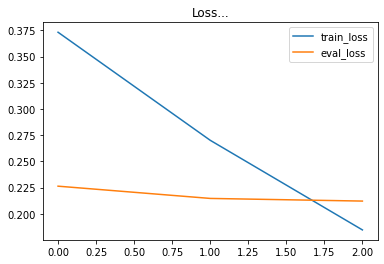
\includegraphics[width= 0.9\linewidth]{gambar/loss_concat_awal.png}
        \caption{Nilai \textit{loss} Acuan}
        \label{fig: loss_baseline}
    \end{center}
\end{figure}

\begin{figure}[h]
    \begin{center}
        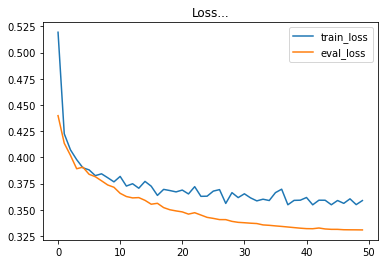
\includegraphics[width= 0.9\linewidth]{gambar/loss_freeze_50.png}
        \caption{Nilai \textit{loss} saat melakukan \textit{training} dengan parameter \textit{freeze}}
        \label{fig: loss_freeze}
    \end{center}
\end{figure}

\begin{figure}[h]
    \begin{center}
        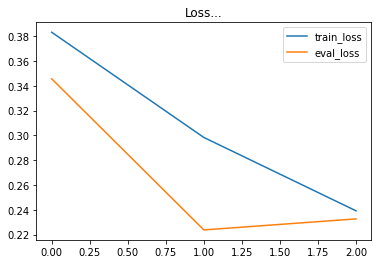
\includegraphics[width= 0.9\linewidth]{gambar/loss_dropout_new.png}
        \caption{nilai \textit{loss} saat melakukan \textit{training} dengan merubah \textit{dropout}}
        \label{fig: loss_dropout}
    \end{center}
\end{figure}

Berdasarkan tabel \ref{tab: model_training_result}, dapat disimpulkan bahwa pada saat melakukan pendekatan berupa parameter \textit{freeze}, waktu \textit{training} menjadi jauh lebih singkat, hal ini karena \textit{optimizer} tidak perlu menghitung ulang \textit{weight} pada setiap \textit{node} dari BERT. Namun, apabila melihat grafik acuan pada gambar \ref{fig: loss_baseline}, terlihat model acuan mengalami sedikit \textit{overfit},  berbeda dengan saat melakukan pendekatan \textit{dropout} dimana grafik \textit{loss} seperti bisa dilihat pada gambar \ref{fig: loss_dropout}, masih menunjukkan grafik yang bagus dan model tidak \textit{overfit} dan memiliki tingkat akurasi yang tidak terpaut jauh dibanding model acuan.